\clearpage
\setcounter{page}{1}
\renewcommand\thesection{\Alph{section}}
\setcounter{section}{0}
\setcounter{footnote}{0}
\setcounter{table}{0}
\setcounter{figure}{0}
\section{Appendix}


\begin{figure*}[t]
\centering
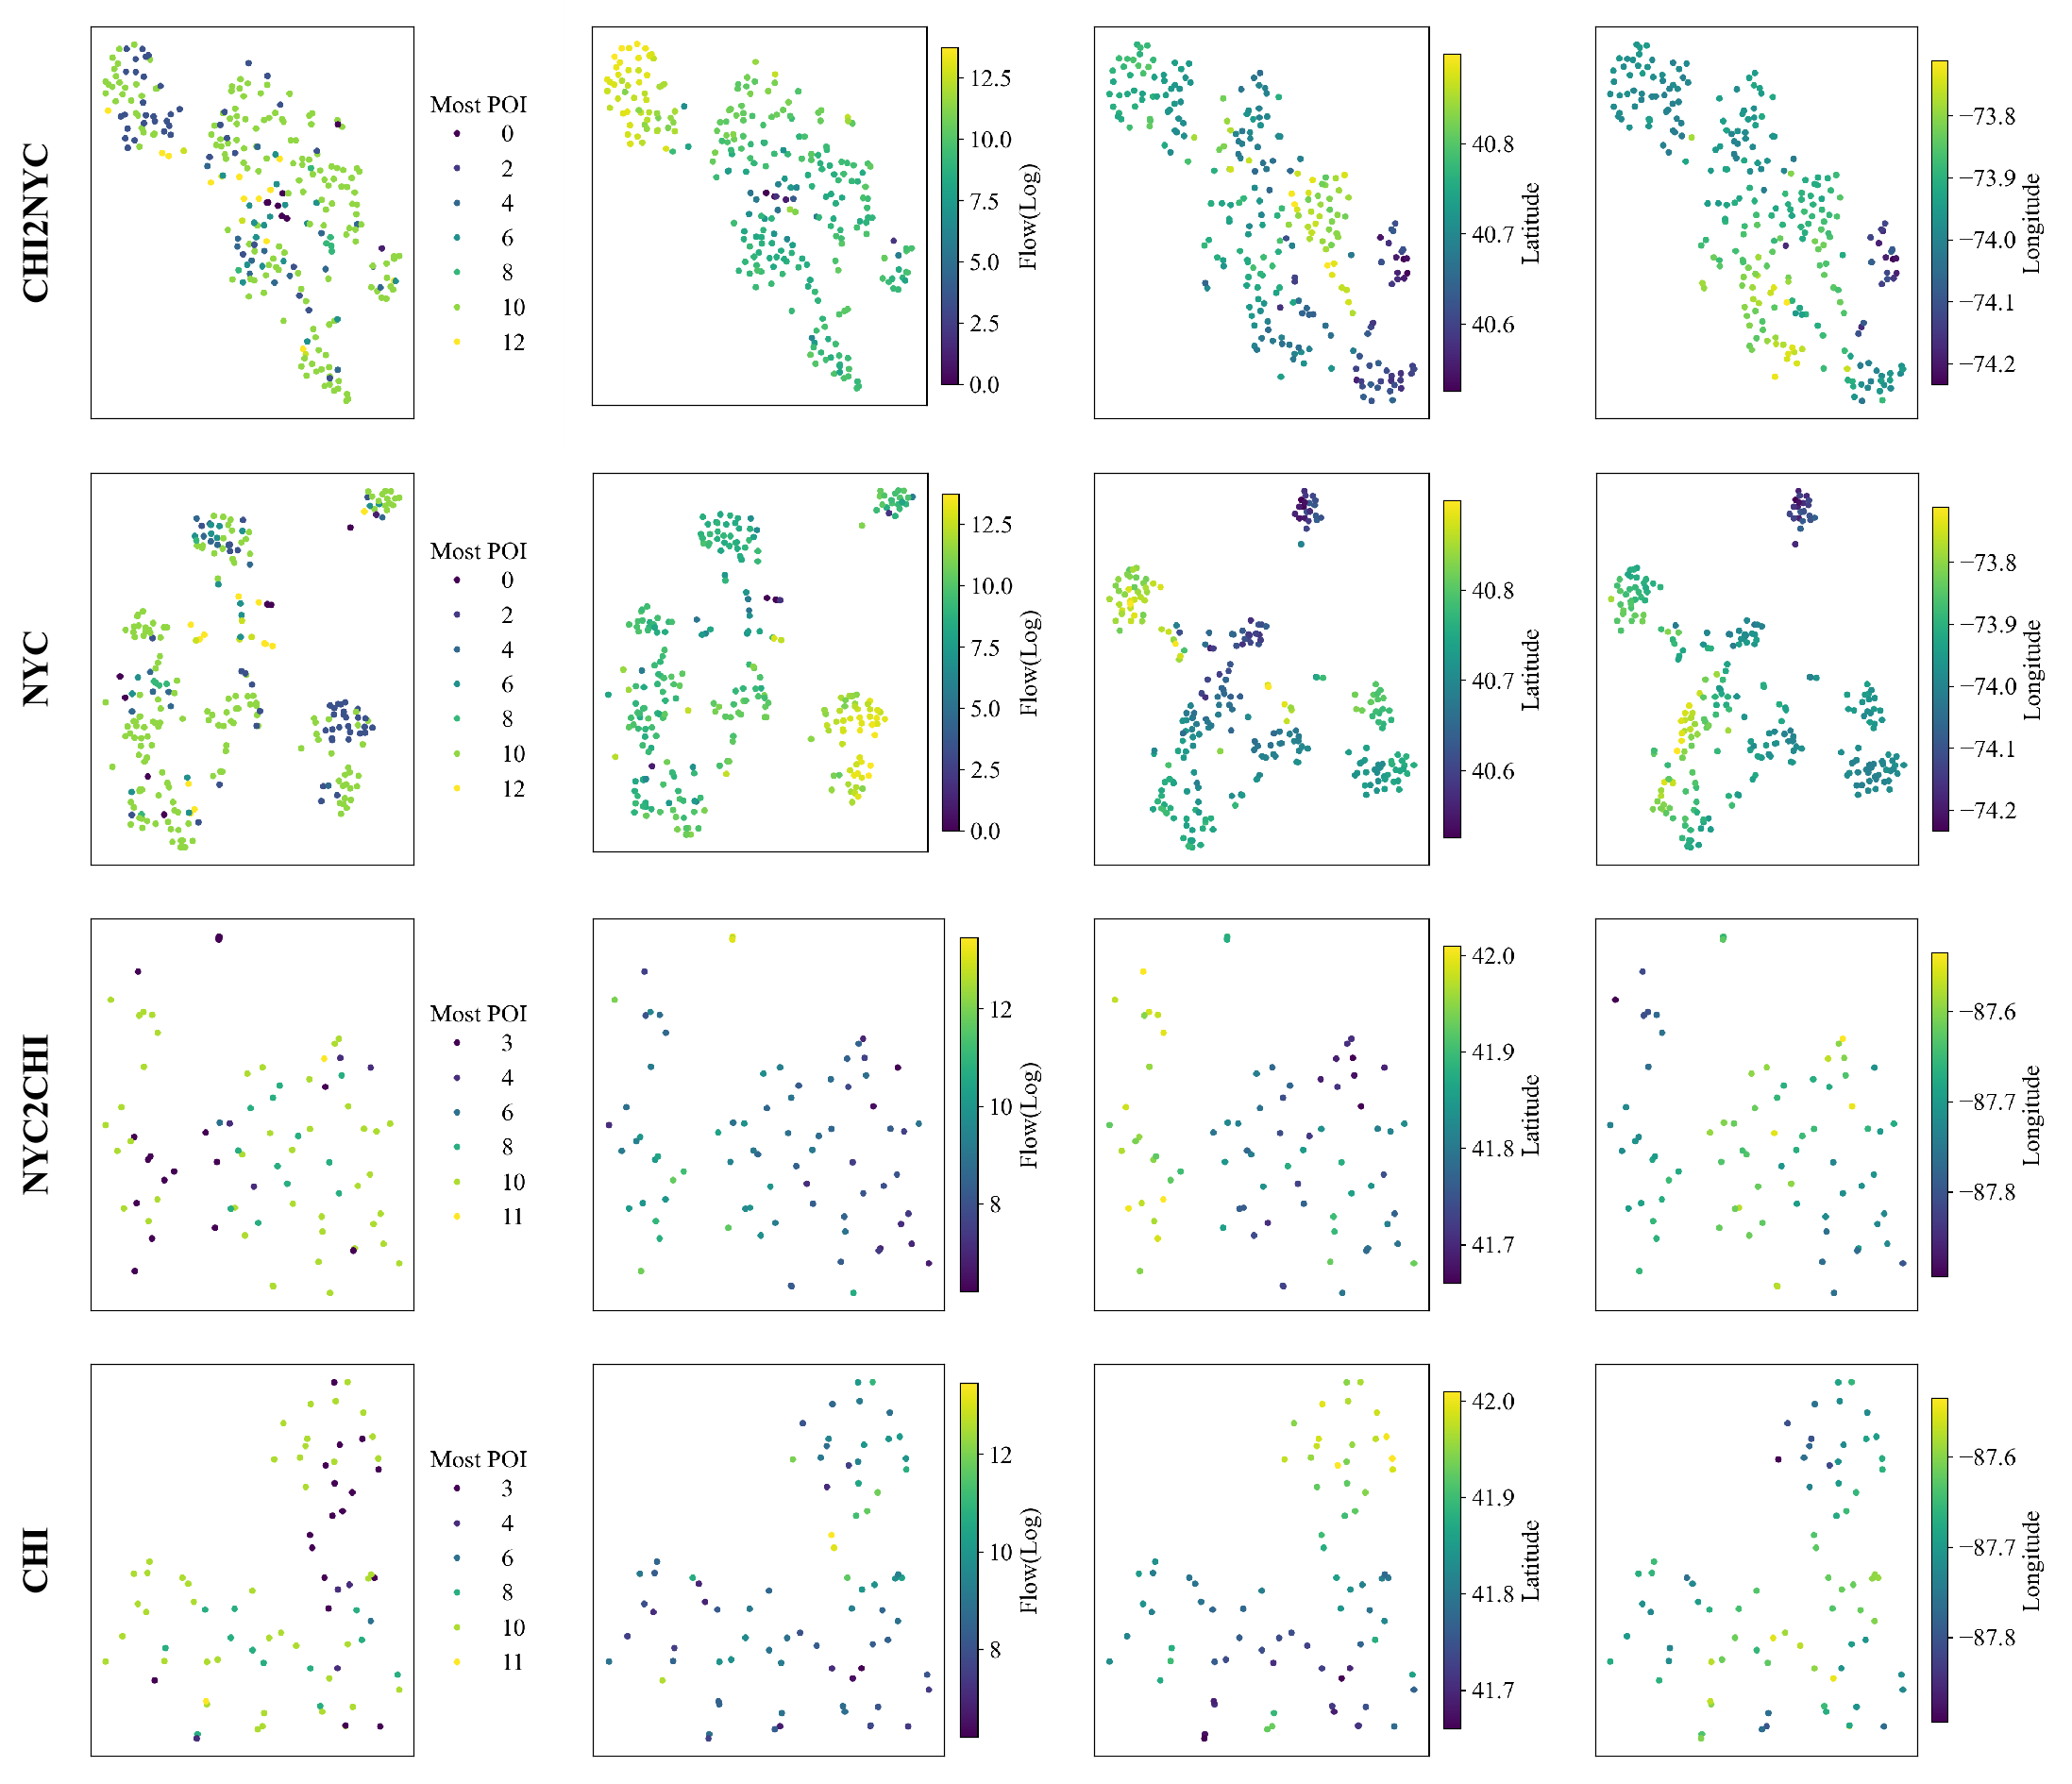
\includegraphics[width=0.99\textwidth]{fig/visualization_v2.png} % Reduce the figure size so that it is slightly narrower than the column.
% 
\caption{Representation Visualization Results in both single-city and cross-city settings}
\label{fig:vr}
\end{figure*}

% 在本章节中，我们对我们的实验设置和可视化结果做出进一步阐释。我们的代码可以在该链接中获取。
In this section, we further explain our experimental setup and visualization results. Our code is available at this link\footnote{https://anonymous.4open.science/r/MAP-STAR-HZX5213}.

\subsection{Datasets}
% 我们的实验主要在New York City(NYC)和Chicago(CHI)两个城市进行。为了在预训练阶段构建heterogeneous subgraph，我们分别收集了两个城市的区域划分、POI和交通流量数据。其中区域划分我们分别采用了NYC TLC\footnote{https://www.nyc.gov/site/tlc\label{fn:tlc}} and CHI Data Portal Community Areas\footnote{https://data.cityofchicago.org\label{fn:CDP}}的划分方式，分别将NYC和CHI分为275个和77个互不重合的网格。POI我们基于OpenStreetMap (OSM)\footnote{https://www.openstreetmap.org/}的数据进行统计。该数据包含POI点的名称（NAME）、类别（CATEGORY）、子类别（SUBCATEGORY）和经纬度（LON, LAT）字段。我们分别基于New York州和Illinois州的数据利用经纬度字段将这些POI点映射到区域中，为每个区域生成一个 $\text{max}_{\text{cate}}$ 维度的一维向量，向量中每个元素代表该区域包含该类别POI的数量。最后将区域间该向量的余弦相似度作为区域之间的POI相似度。此外我们从NYC TLC\footref{fn:tlc}和CHI Data Portal Community Areas\footref{fn:CDP}收集两个城市的出租车记录用于构建人口流动数据。我们收集了从2024.01.01-2024.06.30的出租车乘车记录，将乘车数据聚合为以小时为单位的inflow数据和OD数据as shown in Table \ref{tab:data_statistics}.最终我们基于这三个数据构建heterogeneous subgraphs $\mathcal{G}_i^{\text{sub}}$。

Our experiments are conducted on two major U.S. cities—New York City (NYC) and Chicago (CHI).
During pre-training, we construct heterogeneous subgraphs using three data sources for each city: administrative regions, points of interest (POIs), and taxi mobility records.
\begin{itemize}
    \item \textbf{Administrative regions.} For NYC we adopt the NYC TLC partition\footnote{https://www.nyc.gov/site/tlc\label{fn:tlc}}, and for CHI we use the Community Areas provided by the Chicago Data Portal\footnote{https://data.cityofchicago.org\label{fn:CDP}}. This yields 275 non-overlapping zones in NYC and 77 in CHI.
    \item \textbf{Points of interest.} POIs are extracted from OpenStreetMap (OSM)\footnote{https://www.openstreetmap.org/}. Each POI record contains (NAME, CATEGORY, LON, LAT). Using the coordinates, we assign POIs located in New York State and Illinois State to their corresponding regions, and aggregate them into a $\text{max}_{\text{cate}}$-dimensional vector for every region; each element counts the POIs of a specific category. Cosine similarity between these vectors defines the POI-based similarity between any pair of regions.
    \item \textbf{Taxi mobility.} Taxi trip records are taken from NYC TLC\footref{fn:tlc} and the Chicago Data Portal\footref{fn:CDP}. We collect rides from 2024-01-01 to 2024-06-30 and aggregate them into hourly inflow matrices and origin–destination (OD) matrices (see Table~\ref{tab:data_statistics}).
\end{itemize}
\begin{table}[!htbp]
\centering
    {
        \begin{tabular}{c|ccc}
        \hline
        City     & \#Nodes & \#Time Step    & \#Time Span\\ \hline
        NYC      & 275   & 4368  & 2024.1.1-2024.6.30   \\
        CHI      & 77    & 4368  & 2024.1.1-2024.6.30   \\
        \hline
        \end{tabular}
    }
    \caption{Statistics of pretrain datasets.}
    \label{tab:data_statistics}
\end{table}
Finally, the three data sources are integrated to construct the heterogeneous subgraphs $\mathcal{G}_i^{\text{sub}}$ used throughout this study.

% 为了验证上游预训练表征能够捕获丰富的区域语义信息，并用于各项Urban Computing的任务中，我们从NYC Open Data\footnote{https://opendata.cityofnewyork.us/data/} 和 CHI Data Portal\footref{fn:CDP}中收集了crime和crash两个下游任务的数据。此外我们还基于NPP-VIIRS-like NTL data \cite{DVN/YGIVCD_2020}的数据收集了nightlight下游任务的数据。具体来说，我们筛选了发生在from 2024-01-01 to 2024-06-30时间内的crime和crash，分别在NYC和CHI筛选得到了超过129000条和125000条的crime记录与超过42000条和54000条的crash记录，并基于记录中事件发生的经纬度将这些记录聚合到region中。而NPP-VIIRS-like NTL data按照1km*1km的grid记录了全球nightlight数据，我们基于grid的中心点筛选在每个区域内的网格计算平均nightlight作为该网格的nightlight预测数据。最终构建形成三个下游任务数据。
To evaluate whether the upstream pre-training representations capture rich regional semantics that generalize to diverse Urban Computing tasks, we curate three downstream datasets, crime, crash, and night-light.
\begin{itemize}
    \item \textbf{Crime and crash.} Incident reports are obtained from NYC Open Data\footnote{https://opendata.cityofnewyork.us/data/} and the Chicago Data Portal\footref{fn:CDP}. We select all records that occurred between 2024-01-01 and 2024-06-30, yielding more than 129{,}000 crime events and 42{,}000 traffic crashes in NYC, and over 125{,}000 crime events and 54{,}000 crashes in CHI. Each record is geocoded to latitude–longitude coordinates and then aggregated to its corresponding region.
    \item \textbf{Night-light.} We extract nocturnal luminosity from the NPP-VIIRS-like NTL dataset~\cite{DVN/YGIVCD_2020}, which reports global night-light intensity on a 1,km × 1,km grid. For every region, we average the intensities of all grid cells whose centroids fall within the region boundary, producing the regional night-light target. 
\end{itemize}
% These procedures result in three downstream datasets used to assess the semantic quality of cross-city region embeddings.



\subsection{Baselines}

We compare MAP-STAR with nine state-of-the-art baselines drawn from three methodological groups and evaluate them under two experimental protocols. In the single-city scenario, MAP-STAR is assessed against classical graph-based region representation methods. In the cross-city scenario, we additionally benchmark MAP-STAR against sequence-based and region transfer learning approaches.

\noindent\textbf{Graph-based Region Representation Learning}
\begin{itemize}
\item \textbf{HREP}\cite{HREP}: learns universal region embeddings by constructing heterogeneous relations and prompt-based downstream objectives.
\item \textbf{ReCP}\cite{ReCP}: fuses multi-view data via intra-view contrastive learning plus reconstruction, and inter-view contrastive prediction.
\item \textbf{ST-ReP}~\cite{ST-ReP}: designs multi-scale flow reconstruction and flow-prediction losses to obtain transferable region representations.
\end{itemize}

\noindent\textbf{Sequence-based Methods}
\begin{itemize}
\item \textbf{PatchTST}\cite{PatchTST}: encodes mobility series into patch sequences and exploits a Transformer encoder to model patch-level dependencies.
\item \textbf{TSLANet}\cite{TSLANet}: employs a lightweight CNN-based adaptive network and Fourier transforms to capture temporal and frequency features.
\item \textbf{TimesURL}~\cite{TimesURL}: applies frequency–temporal data augmentation and instance-level contrastive learning for robust flow representations.
\end{itemize}



\noindent\textbf{Region Transfer Learning}
\begin{itemize}
\item \textbf{TransGTR}\cite{TransGTR}: introduces a structure generator that minimizes spatial feature discrepancies between source and target cities.
\item \textbf{CrossST}\cite{CrossST}: builds a Spatial–Temporal Pattern Bank on the source city to transfer the learned urban knowledge.
\item \textbf{CoRE}~\cite{CoRE}: aligns representation manifolds of two cities to transfer mobility knowledge.
\end{itemize}




\subsection{Experimental Implementations}
During pre-training, the input sequence is divided into patches of length 2016 using a sliding window of 168. OD matrices are calculated for the corresponding intervals to facilitate heterogeneous subgraph sampling. For each region node we sample its second-order neighborhood, selecting five first-order and five second-order neighbours to preserve a balanced local topology. For downstream evaluation, we compute the mean inflow for each region and the associated average OD matrix, which are then fed into the encoder. All experiments use a representation dimension of 128. Both pre-training and evaluation rely on the Adam optimiser with a fixed learning rate of 0.001. Early stopping is employed—with a patience of 30 epochs during pre-training and 50 epochs during evaluation—to ensure stable convergence and reliable performance estimates.

\subsection{Representation Visualization}
% 为了进一步探究MAP-STAR获取的区域表征的质量，我们分别利用在NYC和CHI两个源城市上预训练得到的模型，在single-city和cross-city两个setting上获取模型表征。之后为了可视化该表征是否有从三个视角采样的子图上学习城市有关的知识，我们将表征进行降维，分别以区域most poi, flow, latitude和longitu为label进行表征可视化如图 \ref{fig:vr}。表征可视化结果显示，不同label的表征在降维后形成不同的簇，从中可以看出MAP-STAR能够将区域间的POI相似信息、人口流量特征和地理临近性编码进入pattern-bank中，证明我们预训练表征的有效性。此外，不同的模型在相同城市上编码形成的表征分布具有相似性。例如NYC和CHI2NYC两行中，在利用longitude作为label进行可视化时，我们同样得到紫色的较为离群的簇，这验证了我们模型跨城市迁移的能力。
% To further examine the quality of the representations learned by MAP-STAR, we first pre-train the model on the two source cities, NYC and CHI, and obtain embeddings under both the single-city and cross-city settings. We then project these embeddings into a two-dimensional space and visualize them using four region-level labels, most frequent POI category, population flow, latitude, and longitude. The visualizations are presented in Fig.~\ref{fig:vr}.

% After dimensionality reduction, embeddings with different labels form clearly separated clusters. This indicates that MAP-STAR successfully encodes POI similarity, mobility patterns, and geographic proximity into the pattern bank, confirming the effectiveness of our pre-training strategy. Moreover, the embedding distributions produced by different models on the same target city exhibit similar structures. For instance, in the rows “NYC” and “CHI2NYC,” embeddings coloured by longitude both reveal an outlying purple cluster, demonstrating the model’s ability to transfer knowledge across cities.

To further examine the quality of the representations learned by MAP-STAR, we visualize region embeddings obtained under both single-city and cross-city settings. Specifically, MAP-STAR is pre-trained on NYC and CHI, and embeddings are extracted from models trained on NYC alone as well as models transferred from CHI to NYC. These embeddings are projected into a two-dimensional space using dimensionality reduction techniques for qualitative analysis.

To assess whether heterogeneous subgraph sampling enables the model to capture urban semantics from multiple complementary views, we visualize the embeddings using four region-level labels: most frequent POI category, population flow intensity, latitude, and longitude, as shown in Fig.~\ref{fig:vr}. After dimensionality reduction, embeddings associated with different labels form clearly separated clusters. This clustering pattern indicates that MAP-STAR effectively encodes functional similarity, mobility dynamics, and geographic proximity into a shared representation space.

Moreover, embedding distributions under different training settings exhibit highly consistent structures on the same target city. For example, in both “NYC” and “CHI2NYC” settings, longitude-colored visualizations reveal a similar outlying cluster, corresponding to geographically extreme regions. The preservation of such spatial structures across settings suggests that MAP-STAR learns transferable region representations that remain robust under cross-city distribution shifts.


